\subsection{数据预处理：时间、单位与指定时段}

附件1给出的电价、小区负载与光伏发电预测功率具有不同量纲。为使电价与时段购电量相乘得到费用，我们在建模前统一时间和电量口径；曲线标准化仅用于展示，不改变优化输入的物理单位。具体步骤如下。

第一步是时间口径的统一。附件1的记录间隔为10分钟，而电价以元/kWh计量、功率以kW计量，二者的时间基准不一致。为此我们以10分钟为一个时段，将全天划分为144个时段，把功率类数据折算为时段能量，折算公式为：
\begin{equation}\label{eq:src1}
    Q_{t}=P_{t}\cdot \Delta t,\qquad \Delta t=\frac{10}{60}=\frac{1}{6}\ \text{h}
\end{equation}
其中，$P_t$表示第$t$个时段的功率（kW），$Q_t$表示第$t$个时段的电量（kWh），$t=0,1,\dots,143$。原始00:10记录对应00:00--00:10，24:00记录对应23:50--24:00。结果表保留原列序，模板标签与自然日区间的对应关系见支撑材料中的时间映射表。

第二步是净负荷的折算。储能设备的充放电决策本质上由光伏无法覆盖的负载缺口驱动，故先由负载与光伏预测合成净负荷：
\begin{equation}\label{eq:src2}
    N_{t}=L_{t}-V_{t}
\end{equation}
其中，$L_t$为第$t$个时段的小区负载电量（kWh），$V_t$为第$t$个时段的光伏发电电量（kWh），$N_t$为净负荷电量（kWh）。当光伏发电大于负载时，$N_t<0$表示可供储能吸收的余电，我们在优化输入中保留该负值，并将无储能购电基线取为$[N_t]^+$。

第三步是展示尺度的可比化。为在同一坐标系中观察电价与功率的日内形态，我们仅对作图用的三列数据作标准化处理：
\begin{equation}\label{eq:src3}
    z_{t}=\frac{x_{t}-\bar{x}}{\sigma_{x}+\varepsilon}
\end{equation}
其中，$x_t$为原始序列取值，$\bar{x}$与$\sigma_x$分别为该序列的均值与标准差，$\varepsilon=10^{-12}$用于避免除零，$z_t$为标准化后的无量纲序列。标准化后的日内曲线如图\ref{fig:preprocess1}所示。

\begin{figure}[ht]
  \centering
  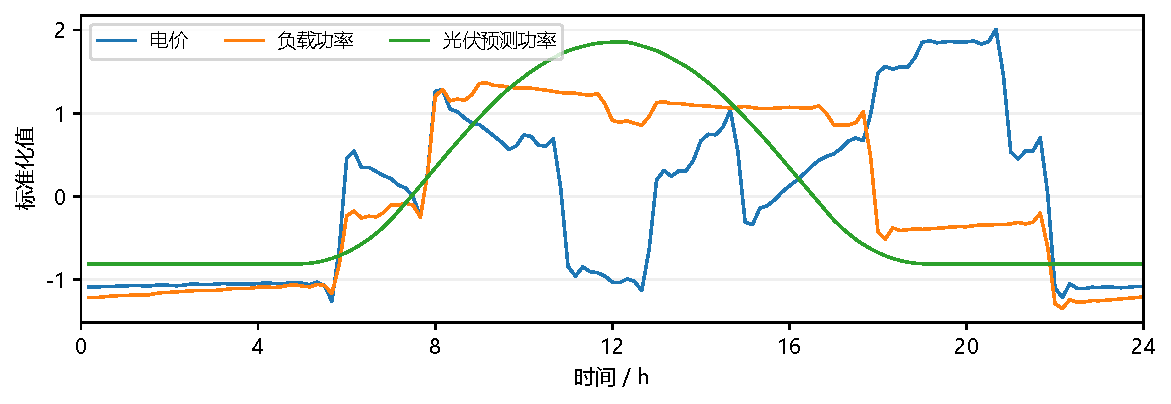
\includegraphics[width=0.72\textwidth]{figures/q1_preprocess.pdf}
  \caption{典型日电价、负载与光伏的标准化曲线}
  \label{fig:preprocess1}
\end{figure}

由图\ref{fig:preprocess1}可知，预处理前电价的数值量级不足功率的百分之一，其日内峰谷结构完全被负载曲线掩盖；标准化后三条曲线处于同一量纲，负载的日内变化、光伏的集中出力时段与电价的峰谷结构均可清晰辨识，为后续以电价为经济杠杆安排充放电时段提供了直观依据。

经上述预处理，我们将本问转化为具有线性目标和线性约束的连续优化问题，并采用线性规划求解。


